\documentclass{standalone}

\usepackage[OT1]{fontenc}
\renewcommand*\familydefault{\sfdefault}
\usepackage{helvet,sfmath}
\usepackage{siunitx}

\usepackage{tikz}
\usetikzlibrary{arrows,calc,patterns}
% \usetikzlibrary{intersections, calc, arrows.meta}
\usepackage{tikz,tkz-euclide}

\definecolor{Liquid1}{RGB}{157, 110, 144}
\definecolor{Liquid2}{RGB}{232, 211, 230}
\definecolor{Note}{RGB}{54, 40, 76}
\definecolor{Rotate}{RGB}{107, 46, 61} 


\begin{document}

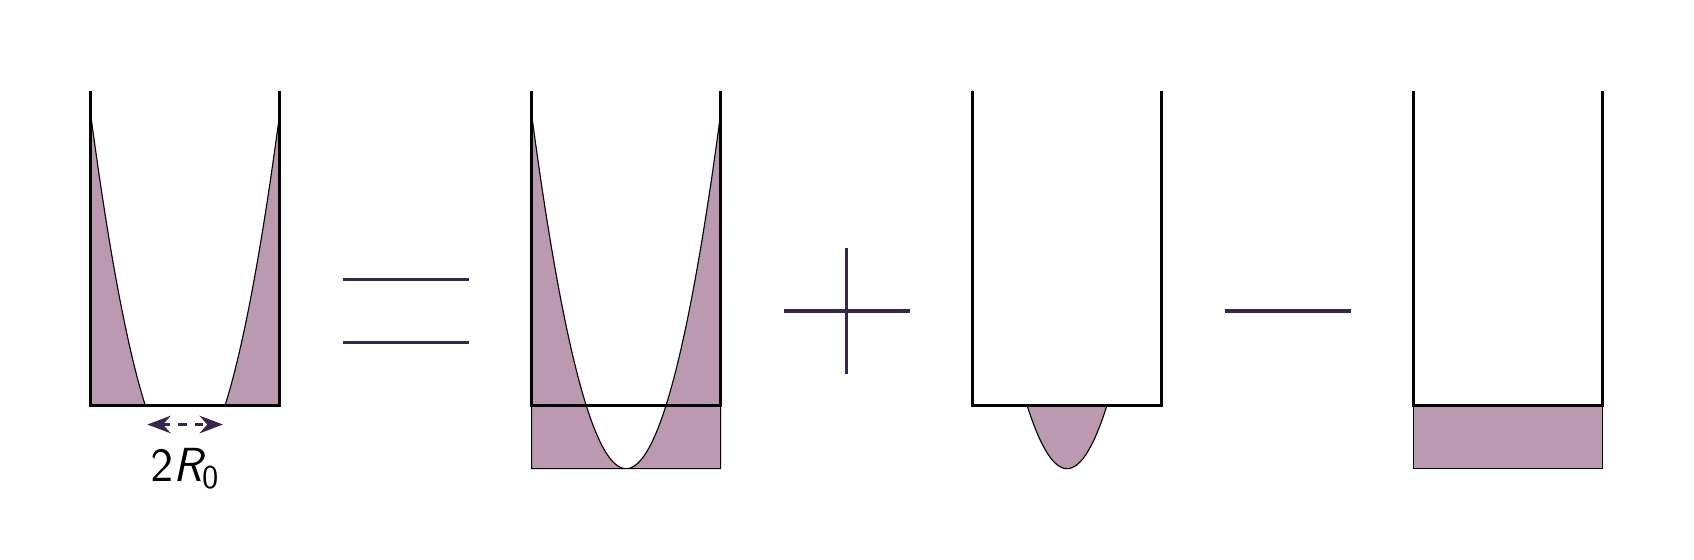
\begin{tikzpicture}[scale=0.8]
    %%Background
    \draw[draw=none] (0,-1) to (26,7);

    %% Initial state
    \draw[fill = Liquid1!70, domain=-1.5:1.5, samples = 200, smooth, variable=\t] 
    plot ({2.5+\t}, {2.5*\t*\t}) to (4,1) to (1,1);
    \draw[draw=none, fill=white] (1,1) rectangle (4,-1);
    \draw[very thick] (1,6) to (1,1) to (4,1) to (4,6);

    %%
    \draw[fill = Liquid1!70, domain=-1.5:1.5, samples = 200, smooth, variable=\t] 
    plot ({9.5+\t}, {2.5*\t*\t}) to (11,0) to (8,0) to (8,1);
    \draw[very thick] (8,6) to (8,1) to (11,1) to (11,6);

    %%
    \draw[fill = Liquid1!70, domain=-1.5:1.5, samples = 200, smooth, variable=\t] 
    plot ({16.5+\t}, {2.5*\t*\t}) to (18,6) to (15,6);
    \draw[draw=none, fill=white] (15,6.1) rectangle (18,1);
    \draw[very thick] (15,6) to (15,1) to (18,1) to (18,6);

    %%
    \draw[fill=Liquid1!70] (22,1) rectangle (25,0);
    \draw[very thick] (22,6) to (22,1) to (25,1) to (25,6);
    
    %%
    %=
    \draw[very thick, Note]
    (5,2) to (7,2)
    (5,3) to (7,3)
    ;
    %+
    \draw[very thick, Note]
    (12,2.5) to (14,2.5)
    (13,1.5) to (13,3.5)
    ;
    %-
    \draw[very thick, Note]
    (19,2.5) to (21,2.5)
    ;

    \draw[Stealth-Stealth, Note, very thick, dashed] (1.9,0.7) to (3.1,0.7);
    \draw (2.5,0) node{\LARGE \(2 R_0\)};
    
\end{tikzpicture}

\end{document}
